
\documentclass[12pt]{article}
\usepackage[cm]{fullpage}
\usepackage[usenames,dvipsnames]{color}
\usepackage{sectsty}
\usepackage{listings}
\usepackage{color}
\usepackage{textpos}
\usepackage[usenames,dvipsnames,table]{xcolor}
\usepackage[small, bf]{caption}
\usepackage{amssymb,latexsym}
\usepackage{amsmath}
\usepackage{xltxtra,xunicode,xgreek}
\usepackage[colorlinks=true, linkcolor = blue, citecolor=blue]{hyperref}
\usepackage[ddmmyyyy]{datetime}
\usepackage{multirow}
\usepackage{tikz}
\usepackage{qtree}
\usepackage{float}
\usepackage{minted}
\usepackage[boxed]{algorithm2e}
\usepackage{textcomp}
\usepackage{fullpage} 
\usepackage{url} 
\usepackage{ocamldoc}


\definecolor{lightgray}{gray}{0.95}
\setmainfont[Mapping=tex-text]{CMU Concrete}
\setmonofont{Courier New}
\newcommand{\tab}{\hspace*{2em}}
\newcommand{\rom}[1]{\uppercase\expandafter{\romannumeral #1\relax}}
\setlength{\parindent}{0pt}
\renewcommand\listingscaption{Κώδικας}

\usemintedstyle{tango}
\SetKw{Kwdto}{downto}

\begin{document}
\begin{titlepage}
\begin{center}


\includegraphics[scale=0.3]{pyrforos.jpg}\\
ΕΘΝΙΚΟ ΜΕΤΣΟΒΙΟ ΠΟΛΥΤΕΧΝΕΙΟ \\
ΣΧΟΛΗ ΗΛΕΚΤΡΟΛΟΓΩΝ ΜΗΧΑΝΙΚΩΝ KΑΙ ΜΗΧΑΝΙΚΩΝ ΥΠΟΛΟΓΙΣΤΩΝ \\ 
\vspace{0.5em}

\medskip 

\def\doubleline{

    \vspace{0.1em}
    \line(1,0){530}\

    \vspace{-1.5em}
    \line(1,0){530}

}
\doubleline
\vspace{1.3em}

{\large \textbf{Στοιχεία Θεωρίας Αριθμών και Εφαρμογές στην Κρυπτογραφία}\\
 \medskip
9ο εξάμηνο, Ακαδημαϊκή περίοδος 2012-2013 \\ \bigskip \medskip}

\vspace{1.5em}
{\LARGE \textbf{Υλοποίηση κρυπτοσυστήματος και ψηφιακής υπογραφής με χρήση ελλειπτικών καμπυλών\\}}
\vspace{32em}

\begin{tabular}{l l}
Νίκος Γιανναράκης & 03108054 \\
Ζωή Παρασκευοπούλου & 03108152 \\
\end{tabular}\\
\bigskip
\today
\end{center}
\end{titlepage}
\tableofcontents

\pagebreak

\section{Ελλειπτικές καμπύλες}

\subsection{Εισαγωγή}
Πολλά συστήματα κρυπτογραφίας βασίζονται σε  πράξεις πάνω σε κάποια αλγεβρική ομάδα. Μπορούμε να χρησιμοποιήσουμε μία ελλειπτική καμπύλη για να ορίσουμε μία ομάδα και έπειτα περιορίζοντας τα σημεία αυτής να ορίσουμε ένα σώμα. Θα δείξουμε αρχικά τις πράξεις που ορίζονται πάνω σε μία τέτοια ομάδα στο πεδίο των πραγματικών αριθμών και μετά στο $\mathcal{F}_p$.
\subsection{Ελλειπτικές καμπύλες στο $\mathcal{R}$}
Μία ελλειπτική καμπύλη στο $\mathcal{R}$ μπορεί να οριστεί ως ένα set σημείων (x,y) που ικανοποιούν μία εξίσωση ελλειπτικής καμπύλης της μορφής: 
$$y^2 = x^3 + a \cdot x + b \; , \; x,y,a,b \in \mathcal{R}$$
Ανάλογα με την επιλογή των a και b έχουμε μία διαφορετική ελλειπτική καμπύλη. Για να ορίσουμε μία ομάδα από μία τέτοια ελλειπτική καμπύλη θα πρέπει το $x^3 + a \cdot x + b$ να μην έχει πολλαπλές ρίζες, δηλαδή να ισχύει $4 \cdot a^3 + 27 \cdot b^2 \neq 0$. Σε αυτή την περίπτωση μία τέτοια ομάδα ορίζεται απο τα σημεία που αποτελούν την ελλειπτική καμπύλη μαζί με ένα ακόμα σημείο $\mathcal{O}$ που θεωρείται το σημείο στο άπειρο.
\subsubsection{Ορισμένες πράξεις σε ελλειπτικές καμπύλες πάνω στο $\mathcal{R}$}
\paragraph{Αντίθετο σημείο}
Αν για δύο σημεία $P = (x_P, y_P)$ και $Q = (x_Q, y_Q)$ ισχύει ότι $Q = (x_P, -y_P)$ τότε λέμε ότι $P = -Q$. Γεωμετρικά αυτό σημαίνει οτι το $Q$ είναι συμμετρικό του $P$ ως προς τον άξονα x.
\paragraph{Πρόσθεση δύο σημείων}
Θα ορίσουμε την πρόσθεση δύο σημείων σε μία ελλειπτική καμπύλη γεωμετρικά. Έστω δύο σημεία $P$ και $Q$ για τα οποία ισχύει ότι $P \neq -Q$. Για να υπολογίσουμε το $R = P + Q$ φέρουμε μία ευθεία που τέμνει και τα δύο σημεία. Η ευθεία αυτή θα τέμνει την καμπύλη σε ακρίβως ένα σημείο ακόμα, το $-R$. Το αντίθετο αυτού είναι το άθροισμα $P+Q = R$. 
Για την περίπτωση όπου $P = -Q$ ισχύει $P + (-P) = \mathcal{O}$.
Επίσης ισχύει ότι $P +\mathcal{O} = P$.

\begin{figure}[H]
\center
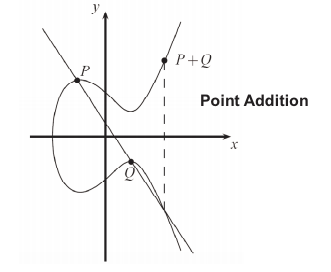
\includegraphics[scale=0.7]{add.png}
\caption{Πρόσθεση δύο σημείων \cite{PAAR}}
\end{figure}

\paragraph{Διπλασιασμός σημείου}
Για την πρόσθεση ενός σημείου $P$ στον εαυτό του φέρουμε ευθεία εφαπτόμενη στο $P$. Αν $y_P \neq 0$ τότε αυτή θα τέμνει την καμπύλη σε ένα ακόμα σημείο, έστω $-R$. Ισχύει ότι $P + P = 2 \cdot P = R$.
Στην περίπτωση που $y_p = 0$ τότε $P + P = 2 \cdot P = \mathcal{O}$.

\begin{figure}[H]
\center
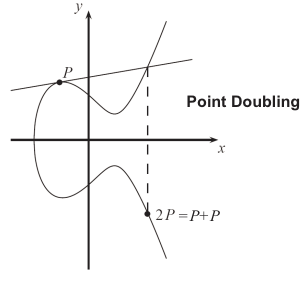
\includegraphics[scale=0.7]{double.png}
\caption{Διπλασιασμός σημείου \cite{PAAR}}
\end{figure}
\subsection{Ελλειπτικές καμπύλες πάνω από το σώμα $\mathbb{F}_p$.}
Οι πράξεις πάνω σε πραγματικούς αριθμούς είναι αργές και στερούνται ακρίβειας λόγω στρογγυλοποιήσεων. Καθώς οι εφαρμογές κρυπτογραφίας απαιτούν ταχύτητα και ακρίβεια στις πράξεις προτιμούνται ελλειπτικές καμπύλες στο σώμα $\mathbb{F}_p$ ή $F_{2^m}$.
Για να ορίσουμε μία ελλειπτική καμπύλη στο $\mathbb{F}_p$ αρκεί να διαλέξουμε $a,b \in \mathbb{F}_p$. Όλα τα σημεία $(x,y)$ της καμπύλης θα ικανοποιούν την εξίσωση αυτής $modulo \; p$.

\subsubsection{Ορισμένες πράξεις σε σε ελλειπτικές καμπύλες πάνω στο $\mathbb{F}_p$}
Μία γεωμετρική προσέγγιση θα αποτύχει σε αυτή την περίπτωση λόγω του πεπερασμένου πλήθους σημείων. Για το λόγο αυτό θα χρησιμοποιήσουμε τις αντίστοιχες αλγεβρικές εξισώσεις.
\paragraph{Αντίθετο σημείο}
Αν για δύο σημεία $P = (x_P, y_P)$ και $Q = (x_Q, y_Q)$ ισχύει ότι $Q = (x_P, -y_P)$ τότε λέμε ότι $P = -Q$. 
\paragraph{Πρόσθεση δύο σημείων}
 Έστω δύο σημεία $P$ και $Q$ για τα οποία ισχύει ότι $P \neq -Q$.
 Έστω ο συντελέστης της ευθείας απο το $P$ στο $Q$ $$s = \frac{(y_P - y_Q)}{(x_P - x_Q)}  \pmod p$$
 Για το $R = P + Q$ θα ισχύει:
 \begin{align*}
 & x_R = s^2 - x_P - x_Q \pmod p \\
 & y_R = -y_P + s \cdot (x_P - x_R) \pmod p
 \end{align*}
 \paragraph{Διπλασιασμός σημείου}
  Αν $y_P \neq 0$ τότε $P + P = 2 \cdot P = R$ όπου το $R$ υπολογίζεται από τις παρακάτω σχέσεις:
  \begin{align*}
  & s = \frac{(3 \cdot x^2_P + a)}{2 \cdot y_P} \pmod p \\
  & x_R = s^2 - 2 \cdot x _P \pmod p \\
  & y_R = -y_p + s \cdot (x_P - x_R) \pmod p
  \end{align*}
\subsection{Ελλειπτικές καμπύλες πάνω από το σώμα $F_{2^m}$.}
  Τα στοχεία του σώματος $F_{2^m}$ είναι m-bit strings για το λόγο αυτό οι υπολογιστές μπορούν να εκτελέσουν αριθμητικές πράξεις πάνω σε αυτά πολύ αποδοτικά. Οι πράξεις δε διαφέρουν από αυτές που ορίσαμε παραπάνω.
 
 \pagebreak
 
\section{Το πρόβλημα του διακριτού λογαρίθμου σε ελλειπτικές καμπύλες (ECDLP)} 
Κάθε σύστημα κρυπτογραφίας βασίζεται σε ένα υπολογιστικό πρόβλημα, συνήθως δύσκολο στον υπολογισμό του απουσία κάποιας πληροφορίας, π.χ. ενός secret key. Μπορούμε να φτιάξουμε συστήματα κρυπτογραφίας που βασίζονται στη δυσκολία υπολογισμού του διακριτού λογάριθμου σε ελλειπτικές καμπύλες (ECDLP).
\subsection{Βαθμωτός Πολλαπλασιασμός}
Ο βαθμωτός πολλαπλασιασμός ενός σημείου $P$ της ελλειπτικής καμπύλης πάνω στο $\mathbb{F}_p$ με έναν ακέραιο $k$ μικρότερο της τάξης του $P$ ορίζεται ώς ένα νέο σημείο $R = k \cdot P = P + P + \cdots + P$ και μπορεί να επιτευχθεί με τις πράξεις πρόσθεσης και διπλασιασμού σημείου που ορίζονται στην ομάδα που ορίζει μια ελλειπτική καμπύλη στο $\mathbb{F}_p$
\subsection{ECDLP}
Με βάση λοιπόν τον βαθμωτό πολλαπλασιασμό ορίζουμε το διακριτό πρόβλημα του λογαρίθμου σε ελλειπτικές καμπύλες ως εξής:

 Έστω $Q = k \cdot P$ όπου $Q, P$ γνωστά σημεία της ελλειπτικής καμπύλης και $k$ ένας ακέραιος. Το $k$ ονομάζεται διακριτός λόγαριθμος του $Q$ στη βάση $P$ και ζητούμενο του προβλήματος είναι ο υπολογισμός του.
\subsection{Elliptic curve Diffie-Hellman (ECDH)}
 Το σχήμα ανταλλαγής κλειδιού Diffie-Hellman για ελλειπτικές καμπύλες ακολουθεί την ίδια λογική με το Diffie-Hellman και στηρίζεται στο ECDLP.
Η διαδικασία που ακολουθείται παρουσιάζεται παρακάτω:
Αρχικά επιλέγονται δημόσια ένα πεπερασμένο σώμα $\mathbb{F}_p$, μία ελλειπτική καμπύλη πάνω σε αυτό το σώμα και ένα σημείο $G$ αυτής (domain parameters).

 Έπειτα οι χρήστες Α και Β κάνουν τα παρακάτω:
\begin{itemize}
\item Επιλέγουν τυχαία έναν αριθμό $d_A$ και $d_B$ αντίστοιχα για τους οποίους ισχύει ότι $d_A < ord(G)$ και $d_B < ord(G)$.
\item Υπολογίζουν το $Q_A = d_A \cdot G$ και $Q_B = d_B \cdot G$ με χρήση βαθμωτού πολλαπλασιασμού.
\item Έχοντας σχηματίσει ένα ζεύγος public-private key $(Q_A,d_A)$ και $(Q_B, d_B)$ αντίστοιχα δημοσιεύουν τα $Q_A, Q_B$.
\item Ο χρήστης Α υπολογίζει το $K = d_A \cdot Q_B$ και ο χρήστης Β το $K = d_B \cdot Q_A$.
\item Έτσι τελικά και οι 2 έχουν υπολογίσει το $K = d_A \cdot d_B \cdot G = d_B \cdot d_A \cdot G$, χωρίς να είναι εφικτό για κάποιον τρίτο να το υπολογίσει χωρίς να λύσει το πρόβλημα του διακριτού λογαρίθμου για ελλειπτικές καμπύλες.
\end{itemize}
\subsection{Elliptic curve digital signature algorithm (ECDSA)}
\paragraph{Παραγωγή υπογραφής}
Για να υπογράψει ένα μήνυμα $m$, ο χρήστης Α με παραμέτρους $D = (q, FR, a, b, G, n, h)$ και ένα ζεύγος ιδιωτικού-δημόσιου κλειδιού $(d, Q)$ ακολουθεί τα παρακάτω βήματα:
\begin{enumerate}
\item Επιλέγει έναν τυχαίο αριθμό $k$ τέτοιο ώστε $1 \leq k \geq n-1$.
\item Υπολογίζει το σημείο $k \cdot G = (x_1, y_1)$.
\item Υπολογίζει το $r = x_1 \pmod n$. Αν $r = 0$ επιστρέφει στο βήμα $1$.
\item Υπολογίζει το $k^{-1} \pmod n$.
\item Υπολογίζει το $SHA-1(m)$ και μετατρέπει το αποτέλεσμα του bit-string σε έναν ακέραιο $e$.
\item Υπολογίζει το $s = k^{-1} \cdot (e + d \cdot r) \pmod n$. Αν $s = 0$ επιστρέφει στο βήμα $1$.
\item Η υπογραφή του A για το μήνυμα $m$ είναι $(r,s)$.
\end{enumerate}

\paragraph{Επαλήθευση υπογραφής}
Για να επαληθέυση μία υπογραφή $(r,s)$ σε ένα μήνυμα $m$, ο χρήστης Β με παραμέτρους $D = (q, FR, a, b, G, n, h)$ και ένα δημόσιο κλειδί $Q$ θα πρέπει αρχικά να επαληθεύσει την ορθότητα των $D$ και $Q$ καθώς μπορεί το $Q$ να έχει τροποποιηθεί απο κάποιον κακόβουλο χρήστη \cite{ECDSA}, έπειτα ακολουθεί τα παρακάτω βήματα:
\begin{enumerate}
\item Επιβεβαιώνει ότι τα $r,s$ είναι ακέραιοι στο διάστημα $[1, n-1]$.
\item Υπολογίζει το $SHA-1(m)$ και μετατρέπει το αποτέλεσμα του bit-string σε έναν ακέραιο $e$.
\item Υπολογίζει το $w = s^{-1} \pmod n$.
\item Υπολογίζει το $u_1 = e \cdot w \pmod n$ και το $u_2 = r \cdot w \pmod n$.
\item Υπολογίζει το $X = u_1 \cdot G + u_2 \cdot G$
\item Εάν $X = \mathcal{O}$ τότε απορρίπτει την υπογραφή. Αλλιώς υπολογίζει τo $u = x_1 \pmod n$ όπου $x_1$ η συντεταγμένη $x$ του $X$. 
\item Δέχεται την υπογραφή αν και μόνο αν $u = r$.
\end{enumerate}
\pagebreak

\section{Υλοποίηση ενός συστήματος κρυπτογραφίας βασισμένο σε ελλειπτικές καμπύλες}
\subsection{Πλεονεκτήματα χρήσης}
Ένας από τους κύριους λόγους χρησιμοποιήσης ελλειπτικών καμπυλών για υλοποίηση συστημάτων κρυπτογραφίας είναι ότι μπορούν να προσφέρουν τον ίδιο βαθμό ασφάλειας με συστήματα όπως το RSA ή το Diffie-Hellman με πολύ μικρότερο μήκος κλειδιού. Έτσι μειώνεται το υπολογιστικό κόστος χωρίς να επηρεάζεται ο βαθμός ασφάλειας. Στον παρακάτω πίνακα παρουσιάζεται το απαιτούμενο μήκος κλειδιού σε bits για το ECC ώστε να επιτευχθεί ανάλογος βαθμός ασφάλειας με αυτή των RSA και AES για διάφορα μήκη κλειδιών.
\\ \medskip


\begin{figure}[!htbp]
\begin{center}
\begin{tabular}{|l|l|l|l|} \hline
\textbf{ECC} & \textbf{RSA} & \textbf{Αναλογία} & \textbf{AES} \\ \hline
163 & 1024 & 1:6 & \\ \hline
256 & 3072 & 1:12 & 128 \\ \hline
384 & 7680 & 1:20 & 192 \\ \hline
512 & 15360 & 1:30 & 256 \\ \hline
\end{tabular} \\
\end{center}
\caption{Αντιστοιχία μήκος κλεδιού σε bits του ECC με RSA και AES}
\end{figure}


Για το λόγο αυτό τα συστήμα κρυπτογραφίας βασισμένα σε ελλειπτικές καμπύλες χρησιμοποιούνται ευρέως σε συσκευές με περιορισμένες υπολογιστικές δυνατότητες και σε συσκευές που απαιτείται χαμηλή κατανάλωση ενέργειας, όπως κινητά για παράδειγμα.

\subsection{Επιλογή παραμέτρων}
Για την αποφυγή επιθέσεων προς το κρυπτοσύστημα απαιτείται κατάλληλη επιλογή των παραμέτρων αυτού.
Οι παράμετροι αυτοί είναι:

\begin{figure}[!htbp]
\begin{center}
\begin{tabular}{|l|l|} \hline
\textbf{Παράμετρος} & \textbf{Περιγραφή} \\ \hline
p & Η χαρακτηριστική του πεπερασμένου σώματος $\mathbb{F}_p$ \\ \hline
a & Ο συντελεστής a της ελλειπτικής καμπύλης \\ \hline
b & Ο συντελεστής b της ελλειπτικής καμπύλης \\ \hline
G & Ένα σημείο $G = (x_G, y_G)$ της ελλειπτικής καμπύλης (base point)  \\ \hline
n & Η τάξη του στοιχείου $G$ \\ \hline
h & $\sharp E(\mathbb{F}_p)/n$ \\ \hline
\end{tabular} \\
\end{center}
\caption{Παράμετροι ECC}
\end{figure}

Οι παραπάνω παράμετροι είναι πολύ σημαντικοί για την ασφάλεια του κρυπτοσυστήματος για αυτό και χρειάζεται ιδιαίτερη μέριμνα στην επιλογή τους. Σχετικά με το ποίες είναι οι επιθυμητές ιδιότητες ασφάλειας των παραμέτρων, πως να παράγουμε παραμέτρους με βάση αυτές και πως να επικυρώσουμε ότι ένα set παραμέτρων έχει τις ιδιότητες αυτές ο αναγνώστης προτρέπεται να ανατρέξει στα \cite{BPOOL}, \cite{SEC2} και\cite{ECDSA}.
Επίσης μπορούμε να χρησιμοποιήσουμε και ένα έτοιμο set παραμέτρων, τακτική που ακολουθήσαμε και εμείς στην υλοποίηση μας με το \emph{brainpoolP256r1} \cite{BPOOL}.

\subsection{Επίπεδα υλοποίησης}
Η υλοποίηση ενός συστήματος κρυπτογραφίας μπορεί να γίνει σε 4 επίπεδα:
\begin{itemize}
\item Στο χαμηλότερο επίπεδο είναι η υλοποίηση modulo αριθμητικής που υπολογιστικά είναι και το πιο ακριβό  μέρος.
\item Υλοποίηση των ορισμένων πράξεων της ομάδας, δηλαδή της πρόσθεσης και του διπλασιασμού σημείου.
\item Υλοποίηση του βαθμωτού πολλαπλασιασμού
\item Στο υψηλότερο επίπεδο είναι η υλοποίηση ενός κρυπτοσυστήματος όπως το ECDH και το ECDSA.
\end{itemize}

\subsection{Αλγόριθμοι υλοποίησης βαθμωτού πολλαπλασιασμού}
Ο πιο απλός τρόπος να υπολογίσουμε το $k \cdot P$ είναι να κάνουμε $k$ προσθέσεις του σημείου $P$ με τον εαυτό του, ωστόσο αυτό δεν είναι καθόλου αποδοτικό.
Για να κατασκευάσουμε ένα αποδοτικό κρυπτοσύστημα χρειαζόμαστε έναν αποδοτικό τρόπο εκτέλεσης βαθμωτού πολλαπλασιασμού.
Ένας αποδοτικός τρόπος είναι με τη μέθοδο double-and-add \cite{PAAR}. \\
%PSEUDOCODE HERE%
\medskip

\begin{algorithm}[H]
\SetAlgoNoLine 
 \KwIn{Elliptic curve $E$, elliptic curve point $P$, scalar $d$:  $(d_1 d_2 \ldots d_t)$ }
 \KwOut{$T = d \cdot P$ }
 $T \leftarrow P$ \\
 \For{$i \leftarrow t -1$ \Kwdto $0$}{
 	$T \leftarrow T + T \pmod n$\\
 	\If{$d_i = 1$}{$T \leftarrow T + P \pmod n$}
 } 
 \KwRet{T}
\caption{Μέθοδος double-and-add}
\end{algorithm}

\bigskip
Υπάρχουν διάφορες παραλλαγές αυτού του αλγορίθμου που στην πράξη είναι πιο αποδοτικοί \cite{BERN}.
\pagebreak
\section{Υλοποίηση στη γλώσσα OCaml}
\subsection{Υλοποίηση βιβλιοθήκης}
Προκειμένου να υλοποιήσουμε ένα σύστημα κρυπτογραφίας βασισμένο σε ελλειπτικές καμπύλες  υλοποιήσαμε μία βιβλιοθήκη που περιέχει όλες τις απαιτούμενες συναρτήσεις.
\subsubsection{Modulo αριθμητική}
Οι πράξεις modulo είναι το πιο ακριβό υπολογιστικά κομμάτι ενός συστήματος κρυπτογραφίας. Για το λόγο αυτό οι προσπάθειες βελτίωσης της απόδησης του συστήματος πρέπει να επικεντρωθούν στο κομμάτι αυτό. 
Για τον παραπάνω λόγο για την υλοποίηση modulo αριθμητικής σε μεγάλους αριθμούς προτιμήσαμε τη βιβλιοθήκη μεγάλων αριθμών \href{http://forge.ocamlcore.org/projects/zarith}{Zarith} που βασίζεται στο GMP καθώς διαθέτει αρκετές και αποδοτικές συναρτήσεις λόγω του ότι το GMP είναι υλοποιημένο σε C και αρκετά optimized σε σχέση με την ενσωματωμένη βιβλιοθήκη της OCaml ή κάποια δική μας λύση.
\subsubsection{Υλοποίηση πράξεων ομάδας}
Έχοντας πλέον την υποστήριξη για modulo αριθμητική υλοποιήσαμε τις συναρτήσεις για τις πράξεις που ορίζονται σε μία ομάδα που ορίζει μία ελλειπτική καμπύλη όπως αυτές αναλύθηκαν στο κεφάλαιο 1.3.1.
\subsubsection{Υλοποίηση βαθμωτού πολλαπλασιασμού}
Χρησιμοποιήσαμε τη μέθοδο double-and-add όπως αναλύεται στο 3.4.
\subsubsection{Ψηφιακή υπογραφή}
Για τη διαδικασία υπογραφής και επαλήθευσης ενός μηνύματος ακολουθήσαμε τον αλγόριθμο που ορίζει το ECDSA με τη διαφορά ότι αντι για την προτεινόμενη secure hash function SHA-1 χρησιμοποιήσαμε το MD5.
\\ \medskip
\emph{Σημειώνεται ότι για πραγματικές εφαρμογές θα πρέπει να χρησιμοποιηθεί μία πιο ισχυρή συνάρτηση κατακερματισμού.
}\subsection{Προγράμματα επίδειξης}
\subsubsection{Υλοποίηση ECDH}
Για να υλοποιήσουμε το σχήμα κρυπτογραφίας ECDH όπως αυτό αναλύθηκε στο 2.3 δημιουργήσαμε δύο προγράμματα που χρησιμοποιούν την παραπάνω βιβλιοθήκη, η λειτουργία των οποίων εξηγείται παρακάτω:
\paragraph{Register.} Το πρόγραμμα \emph{register\_dh} δέχεται ως input ένα username και δημιουργεί ένα αρχείο με όνομα \emph{username.pk} που περιέχει το δημόσιο κλειδί του χρήστη και ένα αρχείο με όνομα \emph{username.sk} που περιέχει το ιδιωτικό κλειδί του χρήστη. Σε περίπτωση που υπάρχουν αρχεία με αυτό το όνομα δίνεται μήνυμα λάθους και το πρόγραμμα τερματίζει. \\
\medskip
\emph{Σημείωνεται ότι το ιδιωτικό κλειδί του χρήστη αποθηκεύεται στο δίσκο ως plain-text,  ενώ σε πραγματική εφαρμογή θα έπρεπε να κρυπτογραφείται.}
\paragraph{Exchange.} Το πρόγραμμα \emph{exchange\_dh} δέχεται ως input το όνομα ενός χρήστη και το όνομα του χρήστη με τον οποίο θέλει να ανταλλάξει κλειδί. Στη συνέχεια διαβάζει το δημόσιο κλειδί του δεύτερου χρήστη και το ιδιωτικό κλειδί του πρώτου χρήστη και υπολογίζει το κοινό κλειδί.
\subsubsection{ECDSA}
Για την υπογραφή μηνυμάτων δημιουργήσαμε δύο προγράμματα που χρησιμοποιούν τις συναρτήσεις \emph{sign} και \emph{verify} της βιβλιοθήκης η λειτουργία των οποίων εξηγείται παρακάτω:
\paragraph{Sign.} Το πρόγραμμα \emph{sign} δέχεται ως input το username ενός χρήστη και ένα μήνυμα και δημιουργεί ένα αρχείο με όνομα \emph{username.msg} που περιέχει το μήνυμα και την υπογραφή. Σε περίπτωση που δε βρεθεί το username δίνεται μήνυμα λάθους και το πρόγραμμα τερματίζει.
\paragraph{Verify.} Το πρόγραμμα \emph{verify} δέχεται ως input το username του χρήστη στον οποίο ανήκει το μήνυμα που θέλουμε να επαληθεύσουμε, ανακτά το δημόσιο κλειδί του, βρίσκει το μήνυμα και την υπογραφή απο το αρχείο που έχει δημιουργήσει το \emph{sign} και επαληθεύει την αυθεντικότητα της υπογραφής.
\subsubsection{Πηγαίος κώδικας}
Ο πηγαίος κώδικας για όλα τα παραπάνω βρίσκεται στο \href{https://github.com/zoep/ECC-OCaml}{Github}.
\subsection{Τεκμηρίωση Βιβλιοθήκης}

\begin{ocamldoccode}
{\tt{module }}{\tt{Ecc}}{\tt{ : }}\end{ocamldoccode}
\label{module:Ecc.Ecc}\index{Ecc@\verb`Ecc`}

\begin{ocamldocsigend}


\label{type:Ecc.Ecc.point}\begin{ocamldoccode}
type point =
  | Infinity
  | Point of Z.t * Z.t
\end{ocamldoccode}
\begin{ocamldocdescription}
An elliptic curve point. It is either infinity or a point (x,y).
\end{ocamldocdescription}
\index{point@\verb`point`}


\label{type:Ecc.Ecc.elliptic-underscorecurve}\begin{ocamldoccode}
type elliptic_curve = {\char123}
  p : Z.t ;
  a : Z.t ;
  b : Z.t ;
  g : point ;
  n : Z.t ;
  h : Z.t ;
{\char125}
\end{ocamldoccode}
\index{elliptic-underscorecurve@\verb`elliptic_curve`}
\begin{ocamldocdescription}
The type of domain parameters
\end{ocamldocdescription}

\label{val:Ecc.Ecc.inverse}\begin{ocamldoccode}
val inverse : Z.t -> Z.t -> Z.t
\end{ocamldoccode}
\index{inverse@\verb`inverse`}
\begin{ocamldocdescription}
\textbf{Ecc.inverse a n} inverses the number a modulo n
\end{ocamldocdescription}


\label{val:Ecc.Ecc.verify-underscorerange}\begin{ocamldoccode}
val verify_range : Z.t -> Z.t -> Z.t -> bool
\end{ocamldoccode}
\index{verify-underscorerange@\verb`verify_range`}
\begin{ocamldocdescription}
\textbf{Ecc.verify\_range a l h} returns true if l $\leq$ a $\leq$ h or false otherwise


\end{ocamldocdescription}


\label{val:Ecc.Ecc.is-underscorepoint}\begin{ocamldoccode}
val is_point : point -> elliptic_curve -> bool
\end{ocamldoccode}
\index{is-underscorepoint@\verb`is_point`}
\begin{ocamldocdescription}
Returns true if a point belongs to an elliptic curve or false otherwise


\end{ocamldocdescription}


\label{val:Ecc.Ecc.double-underscorepoint}\begin{ocamldoccode}
val double_point : point -> elliptic_curve -> point
\end{ocamldoccode}
\index{double-underscorepoint@\verb`double_point`}
\begin{ocamldocdescription}
Given a point P on an elliptic curve and the elliptic curve retuns the point 2P 
        on that curve.


\end{ocamldocdescription}


\label{val:Ecc.Ecc.add-underscorepoint}\begin{ocamldoccode}
val add_point : point -> point -> elliptic_curve -> point
\end{ocamldoccode}
\index{add-underscorepoint@\verb`add_point`}
\begin{ocamldocdescription}
Given two points P and Q, both on the same elliptic curve, and the elliptic curve returns 
        P+Q on that curve.


\end{ocamldocdescription}


\label{val:Ecc.Ecc.multiply-underscorepoint}\begin{ocamldoccode}
val multiply_point : point -> Z.t -> elliptic_curve -> point
\end{ocamldoccode}
\index{multiply-underscorepoint@\verb`multiply_point`}
\begin{ocamldocdescription}
Given a point P on an elliptic curve, an integer k and the elliptic curve returns 
        the scalar multiplication kP on that curve.


\end{ocamldocdescription}




\label{val:Ecc.Ecc.integer-underscoreof-underscoreoctStr}\begin{ocamldoccode}
val integer_of_octStr : string -> Z.t
\end{ocamldoccode}
\index{integer-underscoreof-underscoreoctStr@\verb`integer_of_octStr`}
\begin{ocamldocdescription}
Converts an octet string to an intenger. Useful for defining domain parameters.


\end{ocamldocdescription}


\label{val:Ecc.Ecc.brainpool-underscoreP256-underscorer1}\begin{ocamldoccode}
val brainpool_P256_r1 : elliptic_curve
\end{ocamldoccode}
\index{brainpool-underscoreP256-underscorer1@\verb`brainpool_P256_r1`}
\begin{ocamldocdescription}
An elliptic curve used for ECC as defined by Brainpool


\end{ocamldocdescription}


\label{val:Ecc.Ecc.test-underscorecurve}\begin{ocamldoccode}
val test_curve : elliptic_curve
\end{ocamldoccode}
\index{test-underscorecurve@\verb`test_curve`}
\begin{ocamldocdescription}
An elliptic curve with small domain parameters for testing purposes


\end{ocamldocdescription}


\label{val:Ecc.Ecc.random-underscorebig-underscoreint}\begin{ocamldoccode}
val random_big_int : Z.t -> Z.t
\end{ocamldoccode}
\index{random-underscorebig-underscoreint@\verb`random_big_int`}
\begin{ocamldocdescription}
\textbf{Ecc.random\_big\_int bound} returns a random integer in {\tt{1, bound-1}}


\end{ocamldocdescription}


\label{val:Ecc.Ecc.sign}\begin{ocamldoccode}
val sign : string -> Z.t -> elliptic_curve -> Z.t * Z.t
\end{ocamldoccode}
\index{sign@\verb`sign`}
\begin{ocamldocdescription}
\textbf{Ecc.sign message sk curve} where sk is secret key of the user s and curve 
       the public elliptic curve, returns the signature (r, s) of the message.


\end{ocamldocdescription}


\label{val:Ecc.Ecc.verify}\begin{ocamldoccode}
val verify : string -> Z.t * Z.t -> point -> elliptic_curve -> bool
\end{ocamldoccode}
\index{verify@\verb`verify`}
\begin{ocamldocdescription}
\textbf{Ecc.verify message (r, s) pk curve} where pk is the public key of the user
       who signed the message, returns true if the (r, s) is a valid
       signature or false otherwise.


\end{ocamldocdescription}


\label{val:Ecc.Ecc.create-underscorekeys}\begin{ocamldoccode}
val create_keys : elliptic_curve -> point * Z.t
\end{ocamldoccode}
\index{create-underscorekeys@\verb`create_keys`}
\begin{ocamldocdescription}
Creates a tuple (public\_key, secret\_key) where public\_key is a point of
       the curve and secret\_key an integer.


\end{ocamldocdescription}
\end{ocamldocsigend}


\pagebreak

%http://www.ccs.neu.edu/home/riccardo/courses/cs6750-fa09/talks/Ellis-elliptic-curve-crypto.pdf
%http://cgi.di.uoa.gr/~halatsis/Crypto/Bibliografia/Elliptic/koblitz_ecc.pdf
%http://www.certicom.com/index.php/-50-elliptic-curve-groups-and-the-discrete-logarithm-problem
%http://cs.ucsb.edu/~koc/ccs130h/notes/ecdsa-cert.pdf
%https://engineering.purdue.edu/kak/compsec/NewLectures/Lecture14.pdf
%http://wiki.crypto.rub.de/Buch/download/Understanding_Cryptography_Chptr_9---ECC.pdf
%http://www.ecc-brainpool.org/download/Domain-parameters.pdf
\begin{thebibliography}{2} 
\bibitem{ECDSA} Don Johnson, Alfred Menezes, Scott Vanstone, \emph{The Elliptic Curve Digital Signature Algorithm (ECDSA)}, \emph{Certicom Research}.
\bibitem{SEC2} Certicom Research, \emph{SEC 2: Recommended Elliptic Curve Domain Parameters}, September 2000.
\bibitem{BPOOL} Brainpool, \emph{ECC Brainpool Standard Curves and Curve Generation v1.0}, October 2005.
\bibitem{PAAR} Chrisoft Paar, Jan pelzl, \emph{Understanding Cryptography: A textbook for Students and Practitioners}, \emph{Springer}, July 2010.
\bibitem{BERN} Daniel J. Bernstein, Tanja Lange, \emph{Analysis and optimization of elliptic-curve single-scalar multiplication}.
\end{thebibliography}
\end{document}
